\documentclass{beamer}

\usepackage[utf8]{inputenc}
\usepackage{hyperref}
\usepackage{eurosym}
\usetheme{Darmstadt}

\title{Bien commencer à Robotik}
\subtitle{Ou comment ne pas se faire trop souvent taper sur les doigts}
\author{GaG \\ francois.prugniel@esial.net}
\date{Rentrée 2011-2012}


\begin{document}

\begin{frame}
	\titlepage
\end{frame}

\begin{frame}
	\tableofcontents[hideallsubsections]
\end{frame}

\section{La coupe}
\subsection{Règles de base}
\begin{frame}{Règles de base}
	\begin{itemize}
		\item Robot autonome, on enlève la tirette et il se débrouille
		\item Dimensions limitées : 120cm non déployé, 140cm déployé, 35cm de haut, support balise à 43cm
		\item Détection de l'adversaire
		\item Non dangereux pour les utilisateurs ou arbitres (bords tranchant, coins, explosifs, etc.)
		\item Ne doit pas endommager les éléments de jeux
	\end{itemize}
\end{frame}

\begin{frame}{Règlement}
	\begin{itemize}
		\item Thème : La chasse aux trésors
		\item Publication : 24 Septembre
		\item \href{http://www.planete-sciences.org/}{Site de Planete Sciences}
		\item Brainstorming
	\end{itemize}
\end{frame}

\subsection{Déplacement}
\begin{frame}{Déplacement}
	\begin{itemize}
		\item La Ferté-Bernard
		\item Un bus et une voiture
		\item Petite cotisation des membres/supporters (20-25 \euro)
		\item Hébergement sous tente dans un camping et dans un internat de lycée
	\end{itemize}
\end{frame}

\subsection{Rendez-vous}
\begin{frame}{Rendez-vous}
	\begin{itemize}
		\item Fête de la Science
		\item Pré-coupe Arcelor (hypothétique)
		\item La coupe : 16 au 19 Mai
		\item Le 15 Mai le robot DOIT être totalement opérationnel et pleinement testé
		\item Planning idéal
			\begin{itemize}
				\item 24 Septembre : Sortie du règlement
				\item 31 Octobre : Conception terminée
				\item 31 Décembre : Mécanique totalement opérationnelle
				\item 31 Mars : Tout les systèmes opérationnels et communications testées en conditions réelles
				\item 30 Avril : IA de tueur fonctionnelle avec Asserv, Nav, TNI, Balises et tout le tremblement
				\item 19 Mai : Gagner notre place à Eurobot en poutrant RCVA en finale
			\end{itemize}
	\end{itemize}
\end{frame}


\section{Le club}
\subsection{Les pôles}
\begin{frame}{Info-\'Elec}
	\begin{itemize}
		\item S'occupe de la conception et réalisation électronique
		\item S'occupe du code (IA, etc.)
		\item Gère les communications entre les différents composants
		\item Fait rouler le robot
		\item Maintenance des outils informatiques
	\end{itemize}
\end{frame}

\begin{frame}{Méca}
	\begin{itemize}
		\item Conception de la structure du robot
		\item S'occupe de la fabrication et de l'assemblage
		\item Ne pas oublier qu'il faut intégrer l'électronique et les batteries
		\item Vérifie que les règles sur le périmètre et la sécurité sont respectées
	\end{itemize}
\end{frame}

\begin{frame}{Comm}
	\begin{itemize}
		\item Cherche des sponsors
		\item Organise le déplacement
		\item S'occupe du poster pour la coupe
		\item S'occupe des t-shirt
		\item Préparer le matériel pour l'ambiance
		\item Mettre à jour le blog et la page FB
	\end{itemize}
\end{frame}

\subsection{Le bureau}
\begin{frame}{Le bureau}
	\begin{itemize}
		\item Prez (2A) : Chef de projet, il a le dernier mot sur les décisions à prendre
		\item Vice-Prez (1A) : Permet en théorie au Prez de déléguer
		\item Trez (1A) : S'occupe du budget et harcèle le Trez BDE
		\item Secrétaire (1A) : Fait les comptes rendus des réunions
		\item Responsables de Pôle (2A+) : Chacun s'occupe de son équipe
		\item \^Etre membre du bureau, ça pète sur un CV et on peut/doit assister aux réunions du Lundi midi 
	\end{itemize}
\end{frame}


\section{Le matos}
\subsection{Le club}
\begin{frame}{Le local}
	\begin{itemize}
		\item Prêté par l'ESIAL, donc à ne pas pourrir
		\item Pas d'alcool (enfin, pas dans la journée, au milieu du couloir ou en présence de profs)
		\item Garder rangé
		\item Un sac poubelle, ça se remplace AVANT de déborder
		\item Pour ceux qui auront le code, ne pas le transmettre
		\item Le club est responsable de ce qui se passe dans son local et de son matériel !!
	\end{itemize}
\end{frame}

\begin{frame}{Les outils}
	\begin{itemize}
		\item J'utilise un outil, je le remet à sa place
		\item N'utiliser les outils que pour leurs fonctions primaires (un tournevis, ça ne sert pas à remuer de la peinture et un cutter ne sert pas à dessiner sur de l'acier)
		\item Travailler proprement et de façon précise (niveau, mètre, stylo, pied à coulisse, pince)
		\item Apprendre à se servir des outils avant de faire n'importe quoi avec
		\item Utiliser l'huile de coupe !!!!
	\end{itemize}
\end{frame}

\subsection{L'informatique}
\begin{frame}{Les PC}
	\begin{itemize}
		\item Outils de travail : pas fait pour s'occuper avec des jeux flashs
		\item L'imprimante ne sert pas à imprimer vos cours
		\item Ce qui n'a rien à foutre sur les machines du club sera supprimé sans préavis
		\item Garder des fonds d'écran tout public
		\item \'Eteindre les machines qui ne servent pas
		\item PC jukebox
	\end{itemize}
\end{frame}

\begin{frame}{Les Wiki}
	\begin{itemize}
		\item Wiki Git
			\begin{itemize}
				\item Public, accessible par n'importe qui
				\item Doit contenir les documentations des travaux présent sur le dépôts
			\end{itemize}
		\item Wiki privé
			\begin{itemize}
				\item Annuaire des sponsors, comptes fournisseurs
				\item Documentations de tout les travaux du club
				\item Permet de garder une traces des différentes idées envisagé/exploré
			\end{itemize}
	\end{itemize}
\end{frame}

\section{Le dév}
\subsection{Les langages}
\begin{frame}{Les langages}
	\begin{itemize}
		\item Embarqué $\neq$ PC
		\item Mémoire et puissance limitée
		\item Interférences
		\item C/C++, éventuellement Java sur la PandaBoard
	\end{itemize}
\end{frame}

\begin{frame}{Impératifs vs Objets}
	\begin{itemize}
		\item Impératif : très bien pour les petits programmes peu complexes
		\item Objets : idéal pour les gros programmes qui piquent (Asservissement)
		\item Soit l'un, soit l'autre, pas de mixe des deux
	\end{itemize}
\end{frame}

\subsection{Le code}
\begin{frame}{Conventions de codage}
	\begin{itemize}
		\item Code indenté et aéré
		\item Tabulation = 2 espaces
		\item Nom de variables et de fonctions explicite !!
		\item Commentaires, Commentaires, Commentaires, Commentaires
		\item Toujours utiliser des blocs ( \{\} ), même pour les if/for/while d'une seule ligne
	\end{itemize}
\end{frame}

\begin{frame}{Documentation}
	\begin{itemize}
		\item Tout les travaux doivent être documentés
		\item Explications dans le code avec des commentaires
		\item Petit texte explicatif accompagnant le projet (en txt !!)
		\item Documentations complètes et soignées sur le Wiki pour les éléments complexes
	\end{itemize}
\end{frame}

\section{Git}
\subsection{Principe}
\begin{frame}{Principe}
	\begin{itemize}
		\item Gestionnaire de versions à deux niveaux
		\item Permet le travail collaboratif
		\item Permet de revenir en arrière en cas de mauvaise manipulation
		\item Système de branche pour organiser proprement le travail
		\item Mode d'emploi sur le Wiki
	\end{itemize}
\end{frame}

\subsection{Organisation}
\begin{frame}{Branche master}
	\begin{itemize}
		\item Branche principale
		\item Contient les travaux totalement opérationnels, documentés et testés
		\item En théorie, vous n'avez pas à travailler dedans
	\end{itemize}
\end{frame}

\begin{frame}{Les autres branches}
	\begin{itemize}
		\item Une branche par projet
		\item Branche 2010 et 2011 contiennent les travaux de ces deux années
		\item Ne pas hésiter à faire de nouvelles branches pour explorer une piste
		\item Responsable Git : GaG
	\end{itemize}
\end{frame}

\section{Les systèmes}
\subsection{Asservissement}
\begin{frame}{Asservissement}
	\begin{itemize}
		\item Permet de faire rouler le robot
		\item Boucle fermée de contrôle des moteurs
		\item Feedback des encodeurs optiques pour l'odométrie
		\item SIC, Autom, Maths, Code complexe
		\item Besoin d'un ou deux 1A parfaitement formés dessus pour assurer la pérennité
	\end{itemize}
\end{frame}

\subsection{Détection de l'adversaire}
\begin{frame}{Détection de l'adversaire}
	\begin{itemize}
		\item Solution des télémètres ultrasons permet seulement l'homologation, il faut plus
		\item Utilisation de balises pour repérer l'adversaire et transmettre sa position au robot
		\item SIC, Maths, Système répartit (balises de terrain, balise adversaire, robot)
		\item Besoin d'un ou deux 1A pour participer au développement et pouvoir transmettre la connaissance aux futurs membres
	\end{itemize}
\end{frame}

\subsection{Les autres systèmes}
\begin{frame}{La TNI}
	\begin{itemize}
		\item Traitement Numérique de l'Image
		\item Utiliser une caméra pour repérer des éléments dans l'environnement du robot
		\item A adapter chaque année en fonction des couleurs et des éléments de jeu
		\item Attention aux conditions de luminosité particulières de la coupe
	\end{itemize}
\end{frame}

\begin{frame}{Systèmes divers}
	\begin{itemize}
		\item Préhension des éléments de jeux
		\item Différentiation des éléments de jeux
		\item Gestion du temps et de l'énergie
		\item IA
		\item Navigation
		\item Idées "àlacon" si tout le reste fonctionne et que l'on est en avance
	\end{itemize}
\end{frame}

\section{Bonnes pratiques}
\subsection{Le plus important !!}
\begin{frame}{RTFM !!!!!!!!}
	\begin{center}
		
\includegraphics[scale=0.4]{rtfm01.jpg}
	\end{center}
\end{frame}
\begin{frame}{RTFM !!!!!!!!}
	\begin{center}
		
\includegraphics[scale=0.5]{rtfm02.jpg}
	\end{center}
\end{frame}
\begin{frame}{RTFM !!!!!!!!}
	\begin{center}
		
\includegraphics{rtfm03.jpg}
	\end{center}
\end{frame}
\begin{frame}{RTFM !!!!!!!!}
	\begin{center}
		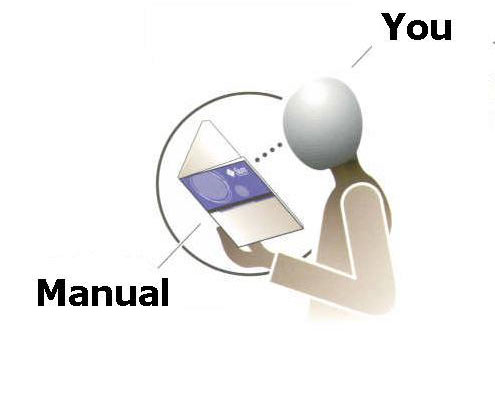
\includegraphics[scale=0.5]{rtfm04.jpg}
	\end{center}
\end{frame}

\subsection{Communications}
\begin{frame}{Les protocoles}
	\begin{itemize}
		\item Série : RS232 ou rien
		\item Bit-à-Bit : Câbles courts et blindés obligatoires
		\item I2C : Relativement robuste aux interférences
		\item TCP : Probablement génial mais difficilement utilisable
		\item USB : Comme TCP
	\end{itemize}
\end{frame}

\begin{frame}{Les interférences}
	\begin{itemize}
		\item Cauchemars du roboticien : J'envoie 01010101, je reçoit 11110000 ou 11001100, etc.
		\item Proviennent des moteurs et des batteries essentiellement
		\item Utiliser des câbles blindés, le plus court possible et passant sur la coque du robot
		\item Condensateur de découplage
		\item Utiliser des ferrites CORRECTEMENT
		\item Trouver le plus de technique possible pour les limiter !! Et les appliquer !!
	\end{itemize}
\end{frame}

\subsection{Le câblage}
\begin{frame}{Le câblage}
	\begin{itemize}
		\item Utiliser des prises robustes avec des détrompeurs
		\item Mettre les prises dans le bon sens pour ne pas avoir à faire sauter les détrompeurs
		\item Marquer ses câbles et ses prises : n'importe qui doit être capable de débrancher/rebrancher une carte sans risque de se tromper
		\item S'assurer que les soudures sont solides, bien faites et isolées : une soudure qui lâche = des heures de recherche pour trouver le problème
		\item Coller des Leds partout, si une carte est sous-tension, elle doit briller !!!
		\item Utiliser des cartes-fusibles partout (régulateur de tension, fusibles, opto-coupleurs, etc.)
		\item Avant de brancher, s'assurer que le câblage est bon, idem pour les tensions !!
	\end{itemize}
\end{frame}

\subsection{Tu peux pas test !!!!!}
\begin{frame}{Tester, Tester, Tester, Tester}
	\begin{itemize}
		\item On ne branche pas sans tester
		\item On test tout, tout le temps, beaucoup
		\item On test à fond, on envisage tout les cas et on les provoquent pour voir ce qui se passe
		\item On test en conditions extrêmes : un protocole de communication n'est viable que s'il fonctionne avec les câbles passant entre les deux moteurs qui tournent à fond !!!
		\item Le robot doit être opérationnel au MINIMUM une semaine avant la coupe pour détecter et corriger toutes les merdes possibles qui vont nous tombez dessus
	\end{itemize}
\end{frame}

\section{Conclusion}
\subsection{Conclusion}
\begin{frame}{Conclusion}
	\begin{itemize}
		\item Ne pas hésiter à poser des questions, même si elles semblent débiles
		\item Seulement et uniquement le manuel détient la vérité : RTFM!!!!
		\item Travaillez régulièrement, même un petit peu, c'est évitez un gros rush à la fin pour finir
		\item Documenter, commenter et coder proprement, c'est assurer la pérennité et moins de temps perdu l'an prochain
	\end{itemize}
\end{frame}

\end{document}